\chapter{Conception}
\label{ch:conception}

\section{La base de données}
\label{sec:database}
Comme des probes requests, des images, et des données personnelles vont être enregistrées et que du traitement
logique leur sera associé, il est important de concevoir une base de donnée claire et bien structurée.

\subsection{Modèle entité-association}
Plusieurs versions du modèle EA ont été imaginées avant d’arriver à la version finale. Afin de mieux cerner les enjeux
de la structure de la base de données, ces dernières vont être commentées. Mais d’abord, listons les différentes
entités

Vendor : Il s’agit du fabricant qui possède un OUI. Étant unique, cet identifiant servira comme clé de la table.

MACAddress : Représente une adresse MAC. Un booléean lui est associé pour savoir si elle semble aléatoire. Une
adresse MAC étant unique (ou presque) elle est utilisée comme clé de la table.

Probe : Représente une probe request. L’heure à laquelle elle a été capturée ainsi que le SSID visé font partie de
l’entité.

Place : Représente l’endroit où la capture a eu lieu.

Picture : Représente une photo prise par le module caméra.

Identity : Représente l’identité d’une personne. On y trouvera les données personnelles récupérées via différents
vecteurs.

BelongsTo: Il s'agit de la relation entre une identité et une MAC adresse. En d'autres mots:
Quelle est la probabilité que la MAC adresse appartienne bien à cette personne ?

Represents: Il s'agit de la relation entre une identité et une image. En d'autres mots:
Quelle est la probabilité que l'image représente bien cette personne ?


\subsubsection{Première version}
Dans cette première ébauche, toutes les entités sont reliées de manière plutôt simpliste. Regardons toutefois
quelques-unes de ces relations.
Une entité « vendor » peut n’avoir délivré aucune adresse MAC puisqu’ils seront tous insérés dans la base de données
à sa création.

Dans ce modèle, visible sur la figure ~\ref{fig:model-ea-1}, une « Identity » est reliée à aucune ou plusieurs MACAddress et photo. (L’individu peut posséder
plusieurs appareils et plusieurs photos ont pu être prises)

\begin{figure}[H]
	\centering
	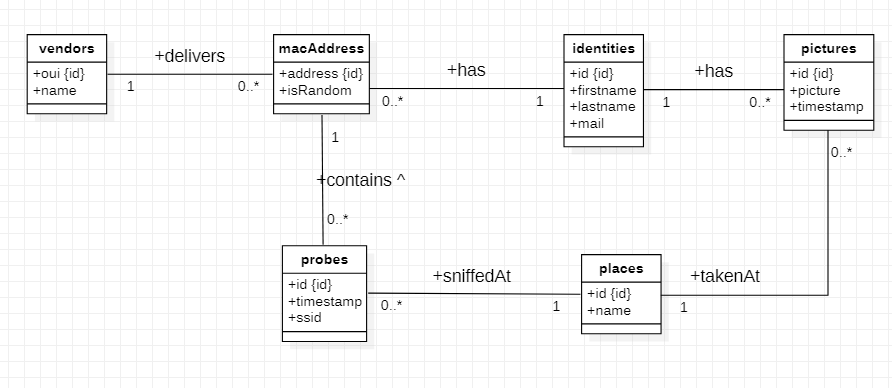
\includegraphics[width=12cm]{images/database_1.png}
	\caption{Première version entité-association}
	\label{fig:model-ea-1}
\end{figure}

Problème : Dans cette conception, il n y a aucune notion de probabilité. Quand une identité a été reliée à une
adresse MAC par exemple, il n’est pas possible de modéliser le doute. Or, dans notre projet, il n y aura que très
peu d'occurences où la certitude est présente. Il faut donc modéliser cette propriété de probabilité.

\subsubsection{Deuxième version – Modélisation des probabilités}
Des relations intermédiaires ont été ajoutées. L’association entre une adresse MAC ou une photo avec une
identité est maintenant « pondérée » par une probabilité. Cette deuxième itération est visible sur la figure ~\ref{fig:model-ea-2}

\begin{figure}[H]
	\centering
	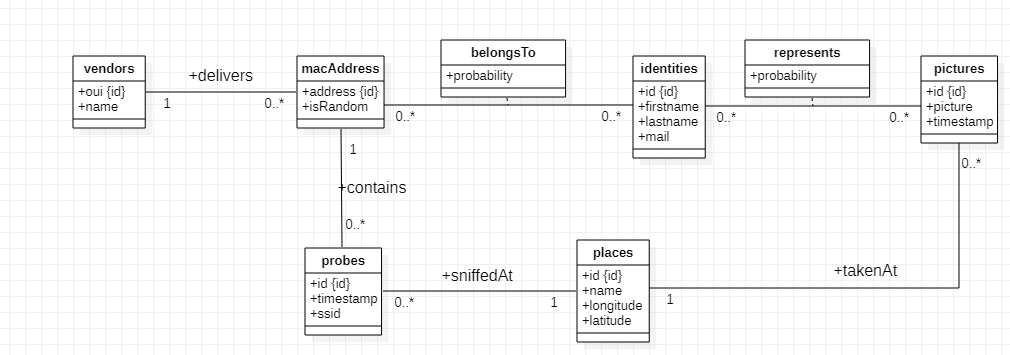
\includegraphics[width=12cm]{images/proto-2.png}
	\caption{Deuxième version entité-association}
	\label{fig:model-ea-2}
\end{figure}

Nouveau problème : Dans ce schéma, il est possible d’obtenir une identité sans image. Or, d’après les
spécifications, ce n’est pas possible puisque c’est grâce à la recherche inversée qu’une identité est établie.

\subsubsection{Troisième version – Identité à partir d’une photographie}

\begin{figure}[H]
	\centering
	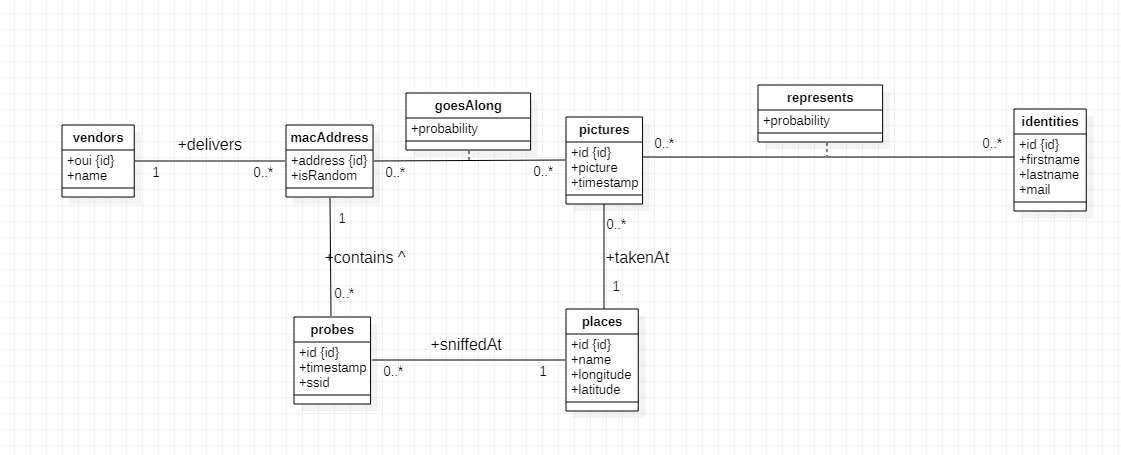
\includegraphics[width=12cm]{images/proto-3.png}
	\caption{Troisième version entité-association}
	\label{fig:model-ea-3}
\end{figure}

Le problème susmentionné a été résolu sur la figure ~\ref{fig:model-ea-3} en détachant l’identité de l’adresse MAC. Seul la photo y est attachée, et
c’est maintenant le lien entre une adresse et une image qui est pondéré.

\subsubsection{Quatrième version – Détails d'une image}

À mi-chemin du projet, il a été remarqué que les données renvoyées par l'API Amazon Rekognition étaient très utiles 
pour implémenter plusieurs fonctionnalités. Ces attributs ont donc été rajoutés à la table Picture.
Ils servent notamment à cibler l'utilisateur (âge, genre, émotions) ou à déterminer la qualité de la photo (sharpness et brightness).
Les nouveaux champs ont été ajoutés sur la figure ~\ref{fig:model-ea-4}

\begin{figure}[H]
	\centering
	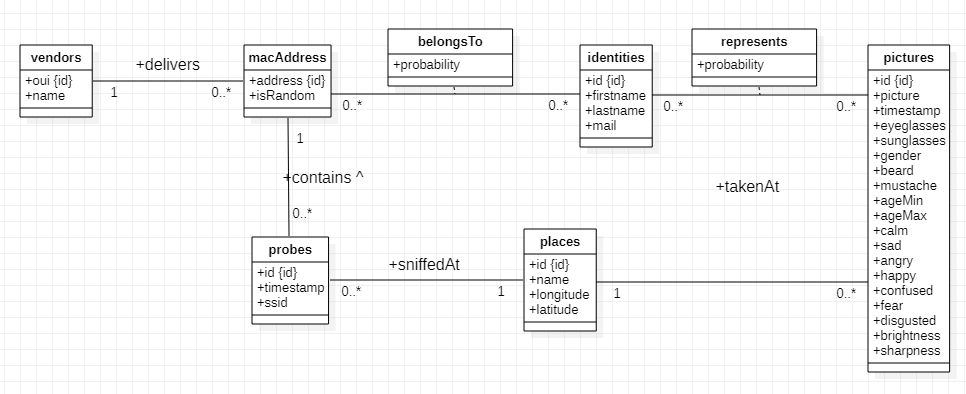
\includegraphics[width=12cm]{images/database_4.png}
	\caption{Quatrième version entité-association}
	\label{fig:model-ea-4}
\end{figure}

\subsubsection{Version finale}

La figure~\ref{fig:model-ea-5} est la version finale du modèle. 
Une entité User a été ajoutée, afin de pouvoir permettre aux clients Raspberry de se localiser.
Un booléean "PP2I" a été ajouté comme attribut de l'entité Identities et MAC Address. Cela permet
d'indiquer si ladite entité doit être incluse dans l'algorithme de mariage PP2I. 

\begin{figure}[H]
	\centering
	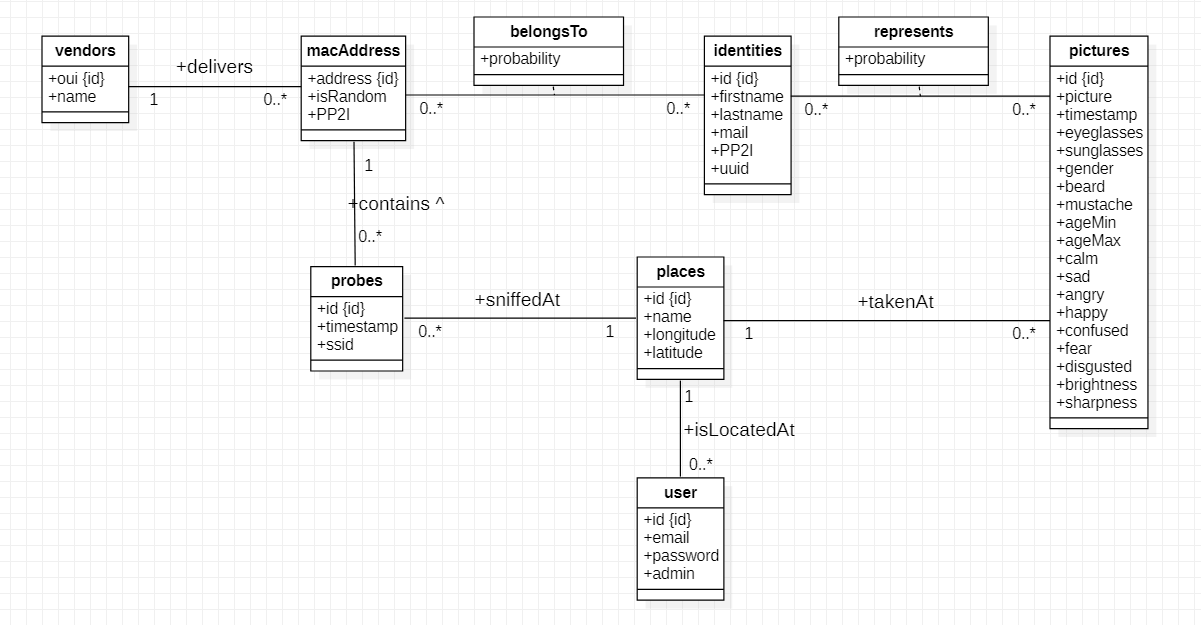
\includegraphics[width=12cm]{images/database_finale.png}
	\caption{Version finale entité-association}
	\label{fig:model-ea-5}
\end{figure}

\section{L'API WiFace}

Afin de développer un projet plus évolutif, sécurisé, et scalable, il a été décidé d'implémenter une API rest permettant les opérations CRUD et d'autres
traitements sur les entités présentées dans la section~\ref{sec:database}.\cite{FLASKREST}
Ainsi, la responsabilité d’effectuer la grande partie de la logique métier pourra
être distribuée au serveur.

Une documentation interactive de toutes les routes est disponible à l'adresse relative \textbf{api/ui} après avoir lancé le serveur~\ref{ch:guide_installation}. 
\section{Le client Raspberry}
Les différents clients Raspberry auront la responsabilité de collecter les informations et de les envoyer
au serveur principal via l'API. 

Pour se faire, elles exécuteront en continu deux processus:
\begin{enumerate}
	\item scanProbe: Récupère les données 802.11 (extraction des MAC Address, du constructeur, analyse de l'aléatoire)
	\item recognizeFace: Analyse des frames de la caméra, si un visage est détecté localement par OpenCV, envoi de l'image à l'API
\end{enumerate}

Ce même client peut être dupliqué autant de fois que nécessaire sans adaptation. 

\section{Dashboard : Visualisation des informations}
Afin qu'un opérateur puisse observer les données récoltées, les données reçues par l'API sont disponibles sous forme de front-end.
Une présentation détaillée des fonctionnalités disponibles est fournie en annexe.

\section{Architecture générale}

L'interaction entre les différents éléments du projet est schématisée sur
la figure~\ref{fig:diag_archi}.

\begin{figure}[H]
	\centering
	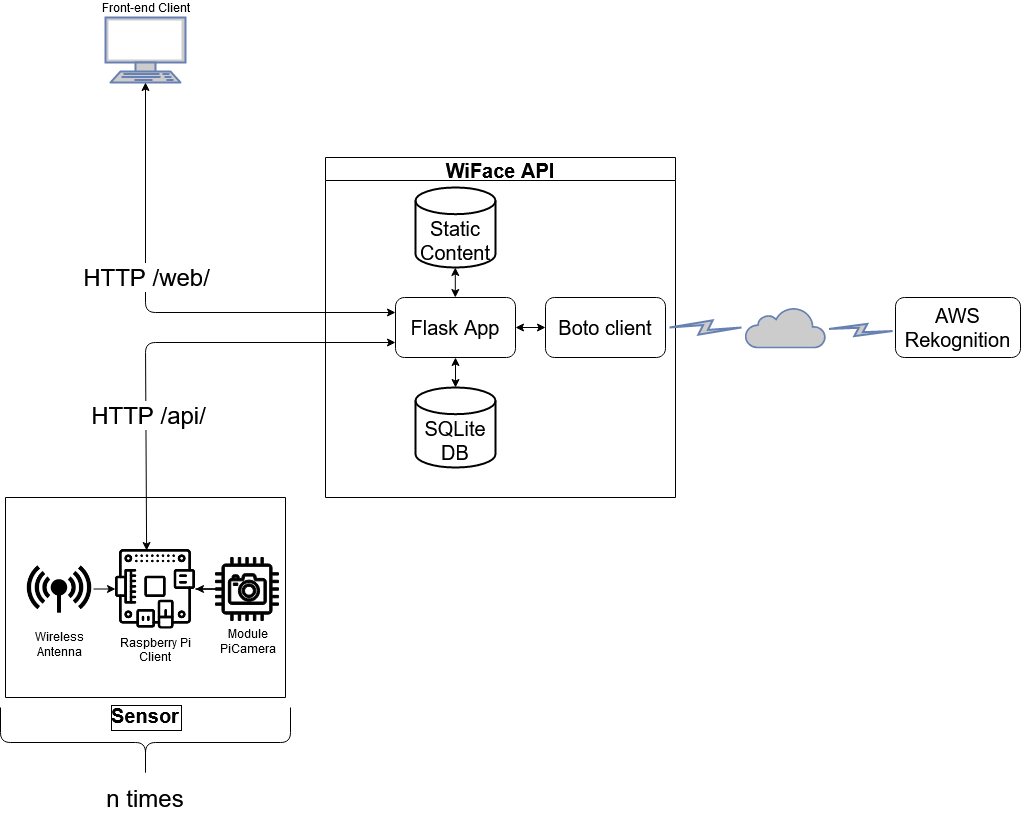
\includegraphics[width=16cm]{images/conception/diagram_archi.png}
	\caption{Diagramme de l'architecture générale}
	\label{fig:diag_archi}
\end{figure}

Les \textbf{sensors} (Client Raspberry Pi, antenne et caméra) s'occupe de récolter les données physiques et de les communiquer à l'API.

Le \textbf{client front-end} peut consulter et gérer les différentes données engrangées par les sensors.

Le point d'entrée de \textbf{l'API WiFace} est \textbf{l'application Flask}. Cette dernière traitera les requêtes
et interagira avec la base de données ou le service Amazon Rekognition si nécessaire.

La \textbf{base de données} permet la persistance des différents éléments (Identités, Utilisateurs, Probe requests récoltées..)

Le \textbf{client "boto"} facilite grandement la communication avec l'API d'Amazon Rekognition, utilisée pour la reconnaissance faciale.


\section{Algorithme PP2I}
L'algorithme PP2I (Probe requests and Pictures to Identity) a la responsabilité d'associer une ou plusieurs adresses MAC à une identité. 
Il a notamment été inspiré d'un travail similaire, sans la composante de reconnaissance faciale.\cite{MACDEAKYN}
Afin d'en analyser le fonctionnement, un lexique doit être établi:
\begin{itemize}
	\item Identité: Personne unique reconnue par l'API Rekognition d'Amazon.
	\item Fenêtre: Intervalle temporel centré autour d'un événement. 
\end{itemize}

Le processus va se dérouler en quatre étapes. 
\begin{enumerate}
	\item Initialisation et incrémentation
	\item Décrémentation majeure dûe à l'absence de l'adresse MAC
	\item Décrémentation mineure dûe à l'absence de la photo
	\item Normalisation des scores
\end{enumerate}

\subsection{Initialisation}
Dans cette phase de l'algorithme, toutes les identités incluses dans l'algorithme (ayant l'attribut PP2I valant True) sont parcourues.
Pour chaque identité, toutes les photos correspondantes sont mises en relation avec probes requests dont l'adresse MAC est inclue dans l'agorithme.
Si un couple (photo, probe request) se trouve dans la même fenêtre, alors on initialise le couple et on l'ajoute au dictionnaire.

\begin{algorithm2e}[H]
	\SetAlgoLined
	\KwIn{List of pictures timestamped and labeled with corresponding identity, list of probe request timestamped}
	\KwResult{Dictionnary containing (adress, identity) tuple as key and probability as value}
	$dict\_couple  \gets \emptyset $\;
	\ForEach(){Identity \textbf{in} AllIdentities}{
		\If(){\textbf{not} Identity.PP2I}{
			$continue$
		}
		 \ForEach(){Picture \textbf{in} Identity}{
			 $beginning \gets Picture.timestamp - half\_window\_duration$\;
			 $end \gets Picture.timestamp + half\_window\_duration$\;
			 $place \gets Picture.place$\;
			 \ForEach(){Probe \textbf{taken at} $place$ \textbf{between} beginning \textbf{and} end \textbf{in} allProbes}{
				\If(){Probe.mac.PP2I}{
			 		$dict\_couple.add(key=(address, identity), value=init\_score)$
			 	}
			}
		}
	}
	\Return{$dict\_couple$}
	\caption{Initialisation et création de couples}
\end{algorithm2e}

\subsection{Décrémentation majeure dûe à l'absence de l'adresse MAC}
Dans cette phase, nous regardons pour un couple donné, si il y a des instances où l'on trouve 
l'identité (une photo) sans l'adresse MAC (une probe request). Comme c'est un cas peu probable si le couple
est correct (une probe request est plus facilement récupérable qu'une photo), on descend beaucoup le score du couple si cela arrive.

\begin{algorithm2e}[H]
	\SetAlgoLined
	\KwIn{$dict\_couple$, list of pictures timestamped and labeled with corresponding identity, list of probe request timestamped}
	\KwResult{Dictionnary containing (adress, identity) tuple as key and probability as value}
	$mac\_addresses  \gets \emptyset $\;
	\ForEach(){Couple \textbf{in} $dict\_couple$}{
		 \ForEach(){Picture \textbf{representing} Couple[Identity]}{
			$beginning \gets Picture.timestamp - half\_window\_duration$\;
			$end \gets Picture.timestamp + half\_window\_duration$\;
			$place \gets Picture.place$\; 
			\ForEach(){Probe \textbf{taken at} $place$ \textbf{between} beginning \textbf{and} end \textbf{in} allProbes}{
				$mac\_addresses.add(Probe.mac)$
			 }
			}
		\If(){Couple[mac] \textbf{not in} $mac\_addresses$}{
			$dict\_couple[(adress, identity)]$ -= $BigMalus$\;
		}

		}
	\Return{$dict\_couple$}
	\caption{Décrémentation majeure dûe à l'absence de l'adresse MAC}
\end{algorithm2e}


\subsection{Décrémentation mineure dûe à l'absence de la photo.}
Dans cette phase, nous regardons pour un couple donné, si il y a des instances où l'on trouve 
l'adresse MAC (une probe request) sans l'identité (une photo). Comme c'est un cas fréquent, on ne baissera qu'un peu le couple donné. 


\begin{algorithm2e}[H]
	\SetAlgoLined
	\KwIn{$dict\_couple$, list of pictures timestamped and labeled with corresponding identity, list of probe request timestamped}
	\KwResult{Dictionnary containing (adress, identity) tuple as key and probability as value}
	$identities  \gets \emptyset $\;
	\ForEach(){Couple \textbf{in} $dict\_couple$}{
		 \ForEach(){Probe \textbf{containing} Couple[address]}{
			$beginning \gets Probe.timestamp - half\_window\_duration$\;
			$end \gets Probe.timestamp + half\_window\_duration$\;
			$place \gets Probe.place$\; 
			\ForEach(){Picture \textbf{taken at} $place$ \textbf{between} beginning \textbf{and} end \textbf{in} allPictures}{
				$identities.add(Picture.identity)$
			 }
			}
		\If(){Couple[identity] \textbf{not in} $identities$}{
			$dict\_couple[(adress, identity)]$ -= $BSmallMalus$\;
		}

		}
	\Return{$dict\_couple$}
	\caption{Décrémentation mineure dûe à l'absence de la photo}
\end{algorithm2e}

\subsection{Normalisation}~\cite{SKLEARNMINMAX}
Afin de faciliter le traitement, les scores seront normalisés dans un interval [0;1].
Pour ce faire, toutes les adresses candidates à une identités sont sélectionnées et mises à l'échelle entre elles à l'aide de la formule suivante:

\begin{listingsbox}{python}{Formule de normalisation}
X_std = (X - X.min) / (X.max - X.min)
X_scaled = X_std * (max_range - min_range) + min_range
\end{listingsbox}